%% Beginning of file 'RNAAS.tex'
%%
%% Modified 2021 April
%%
%%
%% AASTeX v6.31 LaTeX 2e macros.
%%
%% AASTeX is now based on Alexey Vikhlinin's emulateapj.cls 
%% (Copyright 2000-2015).  See the classfile for details.

%% AASTeX requires revtex4-1.cls and other external packages such as
%% latexsym, graphicx, amssymb, longtable, and epsf.  Note that as of 
%% Oct 2020, APS now uses revtex4.2e for its journals but remember that 
%% AASTeX v6+ still uses v4.1.  All of these external packages should 
%% already be present in the modern TeX distributions but not always.
%% For example, revtex4.1 seems to be missing in the linux version of
%% TexLive 2020.  One should be able to get all packages from www.ctan.org.
%% In particular, revtex v4.1 can be found at 
%% https://www.ctan.org/pkg/revtex4-1.

%% The first piece of markup in an AASTeX v6.x document is the \documentclass
%% command.  LaTeX will ignore any data that comes before this command.  The 
%% documentclass can take an optional argument to modify the output style.
%% The command below calls the preprint style which will produce a tightly 
%% typeset, one-column, single-spaced document.  It is the default and thus
%% does not need to be explicitly stated.
%%
%% using aastex version 6.3

\documentclass[12pt,linenumbers]{aastex631}
\newcommand\myfontsizeII{\fontsize{6pt}{12pt}\selectfont}

%% The default is a single spaced, 10 point font, single spaced article.
%% There are 5 other style options available via an optional argument.  They
%% can be invoked like this:
%%
%% \documentclass[arguments]{aastex631}
%% 
%% where the layout options are:
%%
%%  twocolumn   : two text columns, 10 point font, single spaced article.
%%                This is the most compact and represent the final published
%%                derived PDF copy of the accepted manuscript from the publisher
%%  manuscript  : one text column, 12 point font, double spaced article.
%%  preprint    : one text column, 12 point font, single spaced article.  
%%  preprint2   : two text columns, 12 point font, single spaced article.
%%  modern      : a stylish, single text column, 12 point font, article with
%% 		  wider left and right margins.  This uses the Daniel
%% 		  Foreman-Mackey and David Hogg design.
%%  RNAAS       : Supresses an abstract.  Originally for RNAAS manuscripts 
%%                but now that abstracts are required this is obsolete for
%%                AAS Journals.  Authors might need it for other reasons.  DO NOT
%%                use \begin{abstract} and \end{abstract} with this style.
%%
%% Note that you can submit to the AAS Journals in any of these 6 styles.
%%
%% There are other optional arguments one can invoke to allow other stylistic
%% actions.  The available options are:
%%
%%   astrosymb    : Loads Astrosymb font and define \astrocommands.  
%%   tighten      : Makes baselineskip slightly smaller, only works with 
%%                  the twocolumn substyle.
%%   times        : uses times font instead of the default
%%   linenumbers  : turn on lineno package.
%%   trackchanges : required to see the revision mark up and print its output
%%   longauthor   : Do not use the more compressed footnote style (default) for 
%%                  the author/collaboration/affiliations.  Instead print all
%%                  affiliation information after each name.  Creates a much 
%%                  longer author list but may be desirable for short 
%%                  author papers.
%% twocolappendix : make 2 column appendix.
%%   anonymous    : Do not show the authors, affiliations and acknowledgments 
%%                  for dual anonymous review.
%%
%% these can be used in any combination, e.g.
%%
%% \documentclass[twocolumn,linenumbers,trackchanges]{aastex631}
%%
%% AASTeX v6.* now includes \hyperref support.  While we have built in specific
%% defaults into the classfile you can manually override them with the
%% \hypersetup command.  For example,
%%
%% \hypersetup{linkcolor=red,citecolor=green,filecolor=cyan,urlcolor=magenta}
%%
%% will change the color of the internal links to red, the links to the
%% bibliography to green, the file links to cyan, and the external links to
%% magenta.  Additional information on \hyperref options can be found here:
%% https://www.tug.org/applications/hyperref/manual.html#x1-40003
%%
%% Note that in v6.3 "bookmarks" has been changed to "true" in hyperref
%% to improve the accessibility of the compiled pdf file.
%%
%% If you want to create your own macros, you can do so
%% using \newcommand.  Your macros should appear before
%% the \begin{document} command.
%%
\newcommand{\vdag}{(v)^\dagger}
\newcommand\aastex{AAS\TeX}
\newcommand\latex{La\TeX}

\graphicspath{{./}{figures/}}
\usepackage{graphicx}
\usepackage{gensymb}
\usepackage{amsmath}


% FIGSET-MACROS-BEGIN
%\newcommand{\noprint}[1]{}
%\newcommand{\figsetstart}{{\bf Fig. Set} }
%\newcommand{\figsetend}{}
%\newcommand{\figsetgrpstart}{}
%\newcommand{\figsetgrpend}{}
%\newcommand{\figsetnum}[1]{{\bf #1.}}
%\newcommand{\figsettitle}[1]{ {\bf #1} }
%\newcommand{\figsetgrpnum}[1]{\noprint{#1}}
%\newcommand{\figsetgrptitle}[1]{\noprint{#1}}
%\newcommand{\figsetplot}[1]{\noprint{#1}}
%\newcommand{\figsetgrpnote}[1]{\noprint{#1}}
% FIGSET-MACROS-END

%% Reintroduced the \received and \accepted commands from AASTeX v5.2
%\received{March 1, 2021}
%\revised{April 1, 2021}
%\accepted{\today}

%% Command to document which AAS Journal the manuscript was submitted to.
%% Adds "Submitted to " the argument.
%\submitjournal{PSJ}

%% For manuscript that include authors in collaborations, AASTeX v6.31
%% builds on the \collaboration command to allow greater freedom to 
%% keep the traditional author+affiliation information but only show
%% subsets.  The \collaboration command now must appear AFTER the group
%% of authors in the collaboration and it takes TWO arguments.  The last
%% is still the collaboration identifier.  The text given in this
%% argument is what will be shown in the manuscript.  The first argument
%% is the number of author above the \collaboration command to show with
%% the collaboration text.  If there are authors that are not part of any
%% collaboration the \nocollaboration command is used.  This command takes
%% one argument which is also the number of authors above to show.  A
%% dashed line is shown to indicate no collaboration.  This example manuscript
%% shows how these commands work to display specific set of authors 
%% on the front page.
%%
%% For manuscript without any need to use \collaboration the 
%% \AuthorCollaborationLimit command from v6.2 can still be used to 
%% show a subset of authors.
%
%\AuthorCollaborationLimit=2
%
%% will only show Schwarz & Muench on the front page of the manuscript
%% (assuming the \collaboration and \nocollaboration commands are
%% commented out).
%%
%% Note that all of the author will be shown in the published article.
%% This feature is meant to be used prior to acceptance to make the
%% front end of a long author article more manageable.  Please do not use
%% this functionality for manuscripts with less than 20 authors.  Conversely,
%% please do use this when the number of authors exceeds 40.
%%
%% Use \allauthors at the manuscript end to show the full author list.
%% This command should only be used with \AuthorCollaborationLimit is used.

%% The following command can be used to set the latex table counters.  It
%% is needed in this document because it uses a mix of latex tabular and
%% AASTeX deluxetables.  In general it should not be needed.
%\setcounter{table}{1}

%%%%%%%%%%%%%%%%%%%%%%%%%%%%%%%%%%%%%%%%%%%%%%%%%%%%%%%%%%%%%%%%%%%%%%%%%%%%%%%%
%%
%% The following section outlines numerous optional output that
%% can be displayed in the front matter or as running meta-data.
%%
%% If you wish, you may supply running head information, although
%% this information may be modified by the editorial offices.
%\shorttitle{AASTeX v6.3.1 Sample article}
\shortauthors{Reines et al.}
%%
%% You can add a light gray and diagonal water-mark to the first page 
%% with this command:
%% \watermark{text}
%% where "text", e.g.  DRAFT, is the text to appear.  If the text is 
%% long you can control the water-mark size with:
%% \setwatermarkfontsize{dimension}
%% where dimension is any recognized LaTeX dimension, e.g.  pt, in, etc.
%%
%%%%%%%%%%%%%%%%%%%%%%%%%%%%%%%%%%%%%%%%%%%%%%%%%%%%%%%%%%%%%%%%%%%%%%%%%%%%%%%%

%\usepackage{xcolor}
%% This is the end of the preamble.  Indicate the beginning of the
%% manuscript itself with \begin{document}.

\begin{document}

\title{X-RAY OBSCURATION AROUND SUPERMASSIVE BLACK HOLES IN ACTIVE GALAXIES
\footnote{Created: April, 8, 2022}}

%% LaTeX will automatically break titles if they run longer than
%% one line.  However, you may use \\ to force a line break if
%% you desire.  In v6.31 you can include a footnote in the title.

%% A significant change from earlier AASTEX versions is in the structure for 
%% calling author and affiliations.  The change was necessary to implement 
%% auto-indexing of affiliations which prior was a manual process that could 
%% easily be tedious in large author manuscripts.
%%
%% The \author command is the same as before except it now takes an optional
%% argument which is the 16 digit ORCID.  The syntax is:
%% \author[xxxx-xxxx-xxxx-xxxx]{Author Name}
%%
%% This will hyperlink the author name to the author's ORCID page.  Note that
%% during compilation, LaTeX will do some limited checking of the format of
%% the ID to make sure it is valid.  If the "orcid-ID.png" image file is 
%% present or in the LaTeX pathway, the OrcID icon will appear next to
%% the authors name.
%%
%% Use \affiliation for affiliation information.  The old \affil is now aliased
%% to \affiliation.  AASTeX v6.31 will automatically index these in the header.
%% When a duplicate is found its index will be the same as its previous entry.
%%
%% Note that \altaffilmark and \altaffiltext have been removed and thus 
%% can not be used to document secondary affiliations.  If they are used latex
%% will issue a specific error message and quit.  Please use multiple 
%% \affiliation calls for to document more than one affiliation.
%%
%% The new \altaffiliation can be used to indicate some secondary information
%% such as fellowships.  This command produces a non-numeric footnote that is
%% set away from the numeric \affiliation footnotes.  NOTE that if an
%% \altaffiliation command is used it must come BEFORE the \affiliation call,
%% right after the \author command, in order to place the footnotes in
%% the proper location.
%%
%% Use \email to set provide email addresses.  Each \email will appear on its
%% own line so you can put multiple email address in one \email call.  A new
%% \correspondingauthor command is available in V6.31 to identify the
%% corresponding author of the manuscript.  It is the author's responsibility
%% to make sure this name is also in the author list.
%%
%% While authors can be grouped inside the same \author and \affiliation
%% commands it is better to have a single author for each.  This allows for
%% one to exploit all the new benefits and should make book-keeping easier.
%%
%% If done correctly the peer review system will be able to
%% automatically put the author and affiliation information from the manuscript
%% and save the corresponding author the trouble of entering it by hand.

%\correspondingauthor{August Muench}
%\email{greg.schwarz@aas.org, gus.muench@aas.org}

\author[0000-0002-0786-7307]{Abraham J.  Reines}
\author[0000-0002-0786-7307]{Keigo Fukumura}
\affiliation{Physics and Astronomy Department at JMU \\
901 Carrier Dr, Harrisonburg, VA 22807 \\
Harrisonburg, VA 22801, USA}


%\affiliation{Physics and Astronomy Department at JMU\\
%901 Carrier Dr, Harrisonburg, VA 22807 \\
%Harrisonburg, VA 22801, USA}

%\collaboration{6}{(AAS Journals Data Editors)}

%\author{Butler Burton}
%\affiliation{Leiden University}
%\affiliation{AAS Journals Associate Editor-in-Chief}

%\author{Amy Hendrickson}
%\altaffiliation{AASTeX v6+ programmer}
%\affiliation{TeXnology Inc.}

%\author{Julie Steffen}
%\affiliation{AAS Director of Publishing}
%\affiliation{American Astronomical Society \\
%1667 K Street NW, Suite 800 \\
%Washington, DC 20006, USA}

%\author{Magaret Donnelly}
%\affiliation{IOP Publishing, Washington, DC 20005}

%% Note that the \and command from previous versions of AASTeX is now
%% depreciated in this version as it is no longer necessary.  AASTeX 
%% automatically takes care of all commas and "and"s between authors names.

%% AASTeX 6.31 has the new \collaboration and \nocollaboration commands to
%% provide the collaboration status of a group of authors.  These commands 
%% can be used either before or after the list of corresponding authors.  The
%% argument for \collaboration is the collaboration identifier.  Authors are
%% encouraged to surround collaboration identifiers with ()s.  The 
%% \nocollaboration command takes no argument and exists to indicate that
%% the nearby authors are not part of surrounding collaborations.

%% Mark off the abstract in the ``abstract'' environment.  
\begin{abstract}

We investigate obscuration of Active Galactic Nuclei (AGN), identified as Supermassive Black Holes (BH) in luminous galaxies. In this model, winds of plasma particles launched from the accretion disk are photoionized by hard X-ray continua from the AGN's corona, resulting in obscuration in the X-ray band.  Many X-ray spectroscopic observations suggest a majority of AGN are obscured by an intervening gas along our line of sight.  Through photoionization calculations for selected wind solutions, we simulate the observed AGN obscuration distribution.  We discuss the plausibility of the model by comparing our theoretical obscuration distribution to X-ray data by producing a library of synthetic absorption spectra of X-ray continua.  Using our model's obscuration findings, we show how the obscuration distribution is dependent on the model parameters.

\end{abstract}

%% Keywords should appear after the \end{abstract} command.  
%% The AAS Journals now uses Unified Astronomy Thesaurus concepts:
%% https://astrothesaurus.org
%% You will be asked to selected these concepts during the submission process
%% but this old "keyword" functionality is maintained in case authors want
%% to include these concepts in their preprints.
\keywords{AGN Host Galaxies  --- X-ray Active Galactic Nuclei  --- Radiative Magnetohydrodynamics}

%% From the front matter, we move on to the body of the paper.
%% Sections are demarcated by \section and \subsection, respectively.
%% Observe the use of the LaTeX \label
%% command after the \subsection to give a symbolic KEY to the
%% subsection for cross-referencing in a \ref command.
%% You can use LaTeX's \ref and \label commands to keep track of
%% cross-references to sections, equations, tables, and figures.
%% That way, if you change the order of any elements, LaTeX will
%% automatically renumber them.
%%
%% We recommend that authors also use the natbib \citep
%% and \citet commands to identify citations.  The citations are
%% tied to the reference list via symbolic KEYs.  The KEY corresponds
%% to the KEY in the \bibitem in the reference list below.  


\vspace{10pt}
\section{Introduction} \label{sec:intro}
Observational hard X-ray studies suggest the fraction of X-ray obscured AGN decreases with the intrinsic luminosity. The amount of obscured AGN is often described by an absorption function with the obscuring column density, $N_H$.  (Ueda et al., 2003)  \par
We model a Magnetohydrodynamic (MHD) phenomenon responsible for the outflow of plasma particles and ions launched from the accreting disk.  By utilizing magnetized disk wind models, we develop and construct a computational scheme facilitating the calculation of absorption features for AGN hard X-ray spectrum (i.e.  5keV – 50keV).  (Fukumura et al., 2010) Plasma particles and ions flow along magnetic field lines away from the BH accretion disk.  By numerically solving MHD equations for this extreme magnetosphere environment, we validate our model which may explain the physics of the observed surveys of AGN obscuration in the context of accretion disk winds.  We compute a swath of disk-wind solutions for scenarios of varying parameter values.  Our model parameter space includes luminosity - 42 $\leq$ log($L_X$ [ergs$\cdot$s\textsuperscript{-1}]) $\leq$ 46, normalized density of plasma wind - 10\textsuperscript{13} $\leq$ $n_o$ [cm\textsuperscript{-3}] $\leq$ 10\textsuperscript{14}, observation angle - $\theta$ = 30$^{\circ}$, 45$^{\circ}$, 60$^{\circ}$, and power law of transmitted X-ray spectrum - $\Gamma$ = 1.5, 2.0 (X-ray spectra of AGN are described as power law spectra, characterized by the photon index $\Gamma$).
\par
Our method determines the obscuration of hard X-ray photon continuum: the measurement of intervening matter along a line of sight through outflowing disk-wind.  
\hfill
\newpage

\begin{figure}[b]
\centering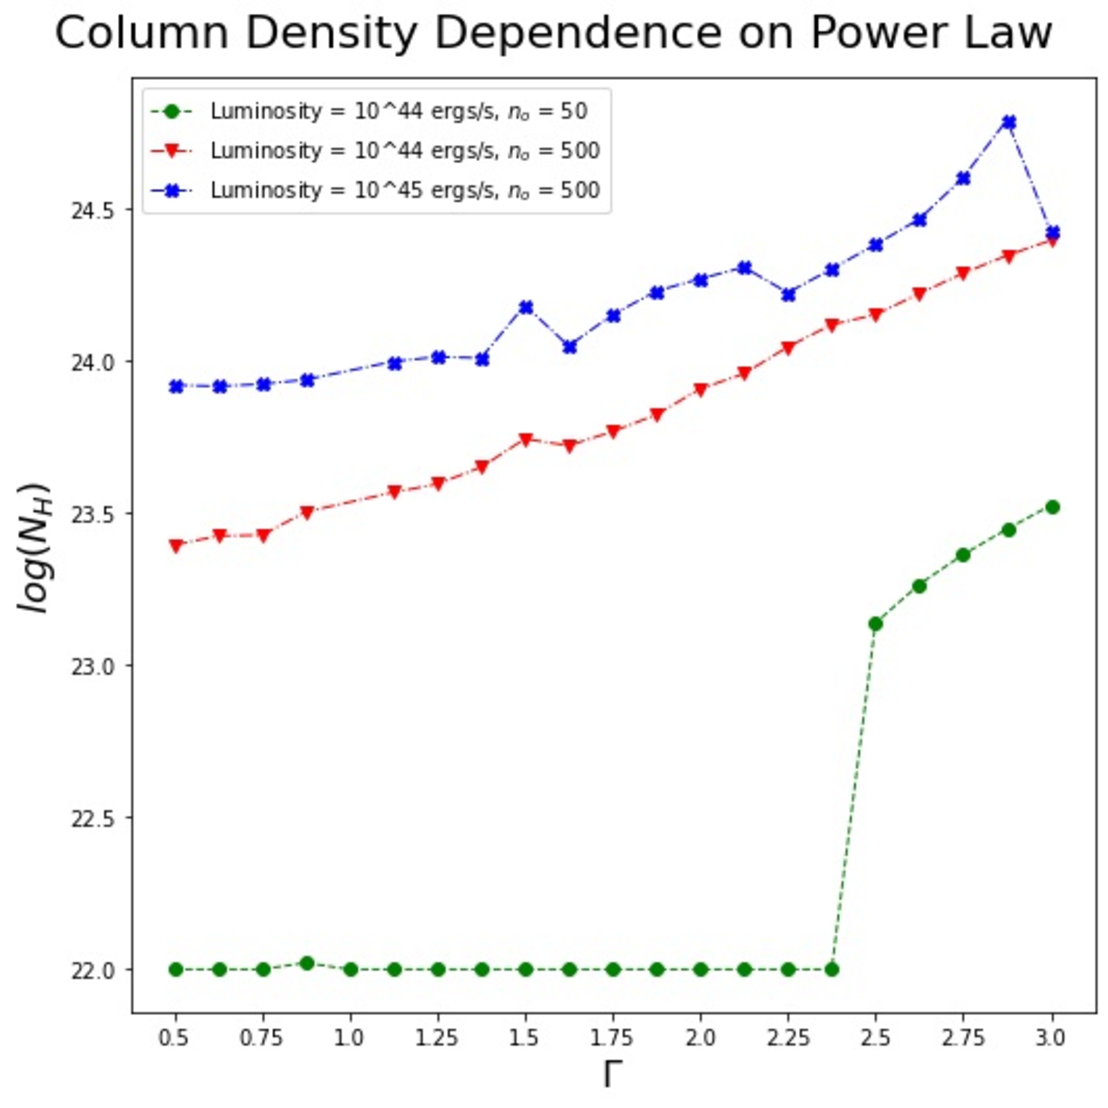
\includegraphics[    page=1,    width=6in,    height=7.50in]{f1_1.pdf}
\caption{Distribution of our synthetic column density for (a) $\Gamma$ = 1.5 and (b) 
%. Bar size indicates number of AGN at designated column density value.  (b) Distribution of our synthetic column density for 
$\Gamma$ = 2.0 along with the luminosity-dependence for (c) $L_X < 10^{43}$, (d) $10^{43} < L_X < 10^{44.5}$ and (e) $10^{44.5} < L_X$.  
%(f) Three regimes of synthetic column density distributions organized by luminosity.  Low luminosity regime (left) contrasts high obscuration found in high luminosity regime (right). The number of less obscured AGN is maintained independent of Luminosity. 
(f) Angular distribution ($\theta$ = 30$^{\circ}$, 45$^{\circ}$, 60$^{\circ}$) of the mean obscuring column densities $N_H$ in our model for three luminosity regimes with the innermost dot being corresponding to (c), the middle dot to (d) and the outermost dot to (e). Color depicts the mean value of $N_H$. Superimposed is the color-coded density distribution (normalized) of the disk-wind.  White vector arrows denote the velocity field, thick curves denote magnetic field lines, and dashed curve for the density contours.   %This plot is the summation of our simulated findings, incorporating $\Gamma$ = 1.5, 2.0. 
}
\end{figure}
\hfill\newpage
\section{Results} \label{sec:style}

	Hard X-ray surveys of a large sample of AGN show many AGN are obscured by a circumnuclear material.  As a result, the observed hard X-ray spectra are partially absorbed by the intervening matter. (Ueda et al., 2003) By conducting radiative transfer process (RTP) calculations using the simulated wind solutions and X-ray radiation from a corona, we show ionized winds launched magnetically from an accretion disk can account partly (if not fully) for the observed obscuration.  For the range of the model parameters (primarily given by X-ray luminosity $L_X$, inclination $\theta$, and wind density $n_o$), we calculate the column density $N_H$ of X-ray-absorbing plasma (i.e.  ionized winds) to construct a distribution of $N_H$ as a function of $L_X$ known as an absorption function.  The calculated absorption function suggests high-inclination AGN (i.e.  larger $\theta$) are obscured the most, while a peak of AGN obscuration exists at the column of $N_H$  $\approx$ 10\textsuperscript{23-24}  cm\textsuperscript{-2} from the luminosity-averaged result.  Our theoretical absorption function is in broad agreement with data from literature, while some quantitative details in the model remain to be improved for better explanation.\par
	Figure 1 (a and b) is a distribution of $N_H$ for individual AGN simulations in units of number per bin, normalized to unity in log($N_H$) = 20 to 24 cm\textsuperscript{-2}; Figure 1a for $\Gamma$ = 1.5 and Figure 1b for $\Gamma$ = 2.0.  Here we illustrate the number of unobscured AGN at $N_H$ of 10\textsuperscript{20} cm\textsuperscript{-2} and highly obscured AGN at $N_H$ of 10\textsuperscript{24} cm\textsuperscript{-2}.  We discovered, using our model simulations, $\Gamma$ has a negligible effect on our obscuration findings: $N_H$.  Our method for plotting our histogram in Figure 1 (a and b) is analogous to distributions of surveys by Ueda et al, 2003.  We identified a vast allotment of essentially unobscured AGN of $N_H$ $\approx$ 10\textsuperscript{5} – 10\textsuperscript{20} cm\textsuperscript{-2}.  Unobscured AGN derive from simulations with low density and luminosity values.  Scenarios with moderate to high luminosity result in greater obscuration of $N_H$ $\approx$ 10\textsuperscript{22} – 10\textsuperscript{24} cm\textsuperscript{-2}.  This is also reflected in observed surveys.  This majority of unobscured AGN have low normalized density and luminosity values.  In the current framework of our model, moderately obscured spectra are the rarest of all populations.  Further research is necessary to understand the physical meaning of this dip.  In our present philosophy, a threshold - particular set of parameter values - exists where highly energetic X-ray photons become absorbed quickly, resulting in the 'gap' illustrated in Figure 1(a and b).  \par
	When examining the upper to lower panels of Figure 1 (c, d, e) we view different luminosity ranges of 42 $\leq$ log($L_X$) $\leq$ 43.5, 43.5 $\leq$  log $L_X$ $\leq$ 44.5, and 44.5 $\leq$ log $L_X$ $\leq$ 46.  As luminosity is raised, we view an increase of obscuration.  Although simple and preliminary (due to limitations of collating and computing the same sample range of AGN), the agreement or our findings with observed surveys is encouraging.  \par
	In Figure 1 (f) we show the predicted angular distribution of obscuring column density (filled dots) in our calculations along with the wind density structure (color-coded) and its contours (dashed curves).  Magnetic field lines are denoted in thick dark curves and wind velocity vector field is given by white arrows.  This cross-sectional view is intended to illustrate the changes in multiple parameters/variables of obscuration phenomenon surrounding the BH. (e.g. Buchner et al., 2015) We examine a geometric distribution of calculated absorption functions.  Each point represents $N_H$ value (in log) averaged over a set of different wind density values at varying $\theta$ (30$^{\circ}$, 45$^{\circ}$, 60$^{\circ}$).  Points closest to the origin correspond to a low luminosity regime.  The set of midpoints correspond to intermediate regime.  The points furthest from origin correspond to high regime.  The contour colors in the background show the wind density distribution as a function of (r, $\theta$) ranging from high (red) near the accretion disk (at  $\theta$ = 90$^{\circ}$) to low (blue) near the innermost wind layer.  \par
	This angular distribution plot illustrates the simple trend of increasing obscuration close to the accretion disk.  The density and luminosity parameters are coupled in the computation of our model.  Therefore, we shall discuss the inverse relation of these parameters, the direct relation of these parameters and the dependence of these parameters on observation angle.  When the normalized density and luminosity are inversely related, density high and luminosity low - and vice versa, $N_H$ is low.  When normalized density and luminosity are directly related at reciprocal high values, $N_H$ is high, as illustrated also by Figure 1c and 1e.  Physically, coronal X-ray photons are absorbed/obscured close to an accretion disk in all luminous AGN.\par
	Notably, obscuration increases with luminosity $L_X$ through the base of the wind at $\theta$ = 60$^{\circ}$.  The wind becomes optically thick with increasing $L_X$, whereas optically thin with decreasing $\theta$ at 30$^{\circ}$ because of the photoionization balance phenomenon.  At low $L_X$ regime, this trend is reversed because the ionization parameter is much lower.  This is our finding in this program.\par



%% For this sample we use BibTeX plus aasjournals.bst to generate the
%% the bibliography.  The sample631.bib file was populated from ADS.  To
%% get the citations to show in the compiled file do the following:
%%
%% pdflatex sample631.tex
%% bibtext sample631
%% pdflatex sample631.tex
%% pdflatex sample631.tex

\newpage
\begin{center}\textbf{This work is supported in part by NASA grant, NNH20ZDA001N-ADAP, and through Astrophysics Data Analysis Program and Jeffress Trust Fund}\end{center}

\section{References}

%\bibliography{sample631}
{Ueda, Y., Akiyama M., Ohta, K.,  Miyaji T., (2003), ApJ, 598:886}\par
{Buchner, J., Georgakakis, A., Nandra, K., Brightman, M., Menzel, M., Lui, Z., Hsu, L., Salvato, M., Rangel, C., Aird, J., Merloni, A.,  Ross, N., (2015), ApJ, 802:89}\par
{Fukumura, K., Kazanas, D., Contopoulos, I. Behar, E. (2010), ApJ, 715, 636}\par
%\bibliographystyle{aasjournal}

%\begin{thebibliography}{777}
%\bibitem{Ueda03} Ueda, Y., Akiyama M., Ohta, K.,  Miyaji T., (2003), ApJ, 598:886
%\bibitem{Buchner15} Buchner, J., Georgakakis, A., Nandra, K., Brightman, M., Menzel, M., Lui, Z., Hsu, L., Salvato, M., Rangel, C., Aird, J., Merloni, A.,  Ross, N., (2015), ApJ, 802:89
%\bibitem{Fukumura10} Fukumura, K., Kazanas, D., Contopoulos, I. Behar, E. (2010), ApJ, 715, 636
%\end{thebibliography}


%% This command is needed to show the entire author+affiliation list when
%% the collaboration and author truncation commands are used.  It has to
%% go at the end of the manuscript.
%\allauthors

%% Include this line if you are using the \added, \replaced, \deleted
%% commands to see a summary list of all changes at the end of the article.
%\listofchanges

\end{document}
